\documentclass[aspectratio=169]{beamer}
\usepackage{preamble_beamer}

\newcommand*{\QEDB}{\null\nobreak\hfill\ensuremath{\square}}

\title[Модель Блэка-Шоулза]{Лекция 4. Модель Блэка-Шоулза} % The short title appears at the bottom of every slide, the full title is only on the title page


\begin{document}

\begin{frame}
\titlepage 
\end{frame}

\begin{frame}{Рекап прошлой лекции} 
\begin{itemize} 
    \item Стохастические дифф. уравнения. Теорема существования, марковость.
    \item Формула Феймана-Каца.
    \item Прямое и обратное уравнение Колмогорова.
\end{itemize}
\end{frame}

\begin{frame}{Динамика портфелей}
    \begin{itemize}
        \item $N$ -- число торгуемых активов (акций)
        \item $h^i_t$ -- число $i$-ых акций на интервале $[t, t + \Delta)$
        \item возможны короткие, длинные и дробные позиции $h^i_t \in \R$
        \item нет транзакционных издержек 
        \item рынок абсолютно ликвиден: нет маркет-импакта
        \item $h_t = [h^1_t, \ldots, h^N_t]$ -- портфель
        \item $S^i_t$ -- цена $i$-го актива в момент $t$
        \item $V_t = \sum_i h^i_t S^i_t = h_t \cdot S_t$ -- капитал портфеля $h$ в момент $t$
        \item Приращение:
        $$
            \Delta V^h_t = V^h_{t + \Delta} - V^h_t = h_t \cdot \Delta S_t + \Delta h_t \cdot S_t + \Delta h_t \cdot \Delta S_t
        $$
    \end{itemize}
\end{frame}

\begin{frame}{Уравнение самофинансируемости}
    \begin{block}{Определение}
        Портфель называется \textbf{самофинансируемым}, если покупка новых активов производится только за счёт продажи старых. 
        \\ Условие самофинансируемости:
        \begin{align*}
            & V^h_{t+\Delta} = h_t \cdot S_{t+\Delta} = h_{t+\Delta} \cdot S_{t+\Delta} \\
            & \Delta V^h_t = h_t \cdot \Delta S_t \\
            & \Delta h_t \cdot S_t + \Delta h_t \cdot \Delta S_t = 0
        \end{align*}
    \end{block}
    При непрерывной торговле $\Delta \to 0$ уравнение самофинансируемости запиывается как:
    $$
        d V^h_t = h_t \cdot dS_t 
    $$
    $$
        V^h_t = V^h_0 + \int_0^t h_u \cdot dS_u
    $$
\end{frame}

\begin{frame}{Модель Блэка-Шоулза}
    Пусть $(\Omega, \mathcal{F}, \mathbb{P})$ -- вероятностное пространство, $W_t$ -- броуновское движение, $(\mathcal{F}_t)_{t\geq 0}$ -- фильтрация, порождённая $W_t$. 
    \pause
    
    Банковский счёт:
    \begin{align*}
        &dB_t = r B_t dt \\
        &B_0 = 1
    \end{align*}\noident Акция:
    \begin{align*}
        &dS_t = S_t \mu dt + S_t \sigma dW_t \\
        &S_t = S_0 \exp\left( \left(\mu - 0.5 \sigma^2 \right) t + \sigma W_t \right)
    \end{align*}
    Динамика самофинансируемого портфеля $h_t = (x_t, y_t)$
    $$
        dV_t^h = x_t dS_t + y_t dB_t = x_t dS_t + (V_t^h - x_t\cdot S_t) r dt 
    $$
\end{frame}

\begin{frame}{Платежные обязательства}
    Пусть $(\Omega, \mathcal{F}, \mathbb{P})$ -- вероятностное пространство, 
    $W_t$ -- броуновское движение, $(\mathcal{F}_t)_{t\geq 0}$ -- фильтрация, порождённая $W_t$.
    \begin{block}{Определение}
        Дериватив -- контракт, который платит в момент $T$ случайную сумму денег $X \in \F_T$.
    \end{block}
    \pause
    \textit{Пример} Европейский колл-опцион: $X = (S_T - K)^+$
    \pause
    \begin{block}{Определение}
        Дериватив называется простым, если $X = \Phi(S_T)$. $\Phi$ -- функция выплаты.
    \end{block}
    \pause
    \textit{Пример} Для европейского колл-опциона $\Phi(x) = (x-K)^+$. \\
    \pause
    \textit{Пример} Азиатский опцион $X = \left( \dfrac{1}{T} \int_0^T S_u du - K\right)^+$ не является простым. 
\end{frame}

\begin{frame}{Общая задача финансовой математики}
    Основная задача -- найти \textit{справедливую} стоимость контракта $p(t, X) \in \F_t$ в произвольный момент времени $t < T$.
\end{frame}

\begin{frame}{Безарбитражность}
    \onslide<1->\begin{block}{Определение}
    Портфель $h$ арбитражный, если 
    $$
        \begin{gathered}
            V^h_0 = 0 \\
            \mathbb{P}(V^h_T \geq 0) = 1 \; \land \; 
            \mathbb{P}(V^h_T > 0) > 0
        \end{gathered}
    $$
    \end{block}

    \onslide<2->{Рынок арбитражный, если существует арбитражный портфель.}
    
    \onslide<3->{
    \textit{Пример}. Пусть 
    $$
        S_t = 1 + W_t^2.
    $$Построить арбитражный порфель.}
\end{frame}

\begin{frame}{Реплицируемый дериватив}
    \begin{block}{Определение}
        Дериватив называется реплицируемым, если $\exists$ самофинансируемый портфель $h_t=(x_t, y_t)$ такой, что:
        $$
            V_T^h \overset{a.s.}{=} \Phi(S_T)
        $$
    \end{block}
    \pause
    \textit{Пример} Пусть $\Phi(S_T) = S_T - K$. Реплицирующий портфель:
    $$
        x_t = 1, \; y_t = -K e^{-rT}
    $$
    \pause
    \begin{block}{Теорема}
        Цена реплицируемого дериватива $\Phi$ равна стоимости реплицирующего портфеля $h_t=(x_t, y_t)$:
        $$
            p(t, \Phi) = V_t^h = x_t S_t + y_t B_t
        $$
    \end{block}
    \pause
    \textit{Пример}.
    $$
        p(t, S_T - K) = S_t - K e^{-r(T-t)}
    $$
\end{frame}

\begin{frame}{Цены}
    \onslide<1->{Пусть $h_t = (x_t, y_t)$ -- самофинансируемый портфель:
        $$
            dV_t = x_t dS_t + (V_t - x_t\cdot S_t) r dt 
        $$
    }
    \onslide<2->{\noident Предположим, что цена $p(t, \Phi) = F(t, S_t)$ -- гладкая функция своих аргументов. Динамика цены:
        \begin{align*}
            &dF(t, S_t) =
            \dfrac{\partial F}{\partial t} dt + \dfrac{\partial F}{\partial S} dS_t + \dfrac{1}{2}\dfrac{\partial^2 F}{\partial S^2} dS_t^2 = \\
            &=\left(\dfrac{\partial F}{\partial t} + 0.5 \sigma^2 S_t^2 \dfrac{\partial^2 F}{\partial S^2}\right) dt + \dfrac{\partial F}{\partial S} dS_t
        \end{align*}
    }
    \onslide<3->{
        Для репликации нужно $dV = dF$. Приравнивая коэф. при $dt, dS_t$ получим:
        \begin{align*}
            &x_t = \dfrac{\partial F}{\partial S},\\
            &\dfrac{\partial F}{\partial t} + r S_t \dfrac{\partial F}{\partial S} + \sigma^2 S_t^2 \dfrac{1}{2}\dfrac{\partial^2 F}{\partial S^2} = r F 
        \end{align*}
    }
\end{frame}

\begin{frame}{Уравнение Блэка-Шоулза}
    \begin{block}{Теорема}
        Пусть $\Phi(S_T)$ -- простой дериватив, тогда его цена $p(t, \Phi) = F(t, S_t)$, где $F(t, S)$ является решением УРЧП:
        \begin{align*}
            &\dfrac{\partial F}{\partial t} + r S \dfrac{\partial F}{\partial S} + \sigma^2 S^2 \dfrac{1}{2}\dfrac{\partial^2 F}{\partial S^2} = r F ,\\
            &F(T, S) = \Phi(S).
        \end{align*}
    \end{block}
    Простой дериватив является реплицируемым, веса реплицирующего портфеля задаются формулами:
    \begin{align*}
        &x_t = \dfrac{\partial F(t, S_t)}{\partial S},\\
        &B_t y_t = F(t, S_t) - \dfrac{\partial F(t, S_t)}{\partial S} S_t.
    \end{align*}
\end{frame}

\begin{frame}{Формула Феймана-Каца}
    \begin{block}{Теорема}
        Пусть функция $F(t, S)$ удовлетворяет УРЧП:
        \begin{align*}
            &\dfrac{\partial F}{\partial t} + r S \dfrac{\partial F}{\partial S} + \sigma^2 S^2 \dfrac{1}{2}\dfrac{\partial^2 F}{\partial S^2} = r F ,\\
            &F(T, S) = \Phi(S).
        \end{align*}
        Тогда решение может быть выраженно через условное мат. ожидание:
        $$
            F(t, S) = \mathbb{E}^Q \left[ e^{-r(T-t)} \Phi(S_T) | S_t = S\right]
        $$где $S_u$ подчиняется геометрическому броуновскому движению:
        \begin{align*}
            &dS_u = r S_u du + \sigma S_u dW_u, u > t \\
            &S_t = S
        \end{align*}
    \end{block}
\end{frame}

\begin{frame}{Риск-нейтральная мера}
    \begin{block}{Определение}
        Мера, относительно которой цена процесса подчиняются уравнению:
        $$
            dS_t = r S_t dt + \sigma S_t dW_t
        $$ называется риск-нейтральной $\mathbb{Q}$.
    \end{block}
    \pause
    \begin{block}{Утверждение}
        Относительно риск-нейтральной меры дисконтированные цены $\widetilde{S_t} = \dfrac{S_t}{B_t}, \widetilde{V_t} = \dfrac{V_t}{B_t}$ мартингалы.
    \end{block}
    \pause
    \textit{Доказательство}. 
    \begin{align*}
        &d \widetilde S_t = \sigma \widetilde S_t dW_t \\
        &d \widetilde V_t = x_t d \widetilde S_t = \sigma x_t \widetilde S_t dW_t 
    \end{align*}
\end{frame}

\begin{frame}{Безарбитражность}
    Формула прайсинга:
    $$
        \dfrac{V_t}{B_t} = \mathbb{E}^{\mathbb{Q}}
        \left[ \dfrac{\Phi(S_T)}{B_T} \mid \mathcal{F}_t\right]
    $$

    \pause 

    \begin{block}{Теорема}
        Модель Блэка-Шоулза безарбитражна. 
    \end{block}
    \textit{Доказательство}. Пусть $(h_t)_{t\geq 0}$ -- арбитражный портфель. Пусть $V_0^h = 0, V_T^h \geq 0$. Тогда:
    $$
        0 = V_0^h = \mathbb{E}^{\mathbb{Q}} \dfrac{V_T^h}{B_T} \to \mathbb{Q}(V_T = 0) = 1
    $$
\end{frame}

\begin{frame}{Пример. Форвард.}
    \begin{block}{Определение}
        Форвардный контракт со страйком $K$ и датой погашения $T$ это случайное платёжное обязательство с функцией выплаты:
        $$
            \Phi(S_T) = S_T - K
        $$
    \end{block}
    
    \pause

    Цена:
    $$
        p(t, S_T - K) = S_t - e^{-r(T-t)} K
    $$

    \pause

    \begin{block}{Форвардная цена}
        Форвардная цена -- страйк, при котором цена форвардного контракта равна нулю:
        $$
            p(0, S_T - K) = 0
        $$
    \end{block}
    $$F = S_0 e^{rT}; p(t, S_T - F) = S_t - S_0 e^{rt}$$    
\end{frame}

\begin{frame}{Пример. Европейский колл-опцион}
    \begin{block}{Определение}
        Европейский колл-опцион со страйком $K$ и датой погашения $T$ это случайное платёжное обязательство с функцией выплаты:
        $$\Phi(S_T) = \max(S_T-K, 0) = (S_T - K)^+$$
    \end{block}

    \pause
    Цена колл-опциона задаётся формулой:
    \begin{align*}
        &C(t, S_t) = S_t N(d_1) - e^{-r\tau}K N(d_2) \\
        &d_1 = \frac{\ln(S_t/K) + (r+0.5\sigma^2)\tau}{\sigma \sqrt{\tau}}\\
        &d_2 = d_1 - \sigma \sqrt{\tau}\\
        & N(x) = \dfrac{1}{\sqrt{2\pi}}\int_{-\infty}^x e^{-u^2/2}du,
    \end{align*}где $\tau=T-t$ -- время до эксперации.
\end{frame}

\begin{frame}{Пример. Европейский колл-опцион}
    \textit{Доказательство}. Введём $\tau = T - t$ -- время до экспирации.
    \begin{align*}
        &C(t, S_T) = e^{-r\tau}\mathbb{E}^{\mathbb{Q}_t}(S_T - K) \mathbb{I}_{S_T \geq K} 
        = \mathbb{E}^{\mathbb{Q}_t}\left[e^{-r\tau} S_T \mathbb{I}_{S_T \geq K}\right] - K e^{-r\tau} \mathbb{Q}(S_T \geq K).
    \end{align*}
    1) Вычислим $\mathbb{Q}(S_T \geq K)$:
        $$
            S_T = S_t e^{(r-0.5 \sigma^2)\tau + \sigma (W_T - W_t)} = S_t e^{(r-0.5 \sigma^2)\tau + \sigma \xi \sqrt{\tau}},
        $$где $\xi \sim N(0, 1)$ -- стандартная нормальная с.в.. 
        \begin{align*}
            &S_T \geq K \longleftrightarrow \\
            &S_t \exp \left[ (r-0.5\sigma^2)\tau + \sigma \xi \sqrt{\tau}\right] \geq K \longleftrightarrow \\
            &  (r-0.5\sigma^2)\tau + \sigma \xi \sqrt{\tau} \geq \log(K / S_t) \longleftrightarrow \\ 
            & \xi \geq - \dfrac{\log(S_t/K) + (r-0.5\sigma^2)\tau}{\sigma \sqrt{\tau}} \overset{def}{=} -d_2.
        \end{align*}
        Итого:
        $$
            \mathbb{Q}(S_T \geq K) = \mathbb{Q}(\xi \geq -d_2) = \mathbb{Q}(\xi \leq d_2) = N(d_2) \qed
        $$
\end{frame}

\begin{frame}{Пример. Европейский колл-опцион}
    2) Вычислим $\mathbb{E}^{\mathbb{Q}_t}\left[e^{-r\tau} S_T \mathbb{I}_{S_T \geq K}\right]$:

    $$
        \mathbb{E}^{\mathbb{Q}_t}\left[e^{-r\tau} S_T \mathbb{I}_{S_T \geq K}\right]  
    = S_t \dfrac{1}{\sqrt{2\pi}}\int\limits_{-d_2}^{\infty} \exp\left[-\dfrac{1}{2} \sigma^2\tau + \sigma x \sqrt{\tau}-\frac{x^2}{2} \right]dx.
    $$

    Рассмотрим отдельно выражение под экспонентой и выделим полный квадрат:
    $$
        -\dfrac{1}{2}\left(\sigma^2 \tau - 2x\sigma \sqrt{\tau} + x^2 \right) = -\dfrac{1}{2} \left(x-\sigma \sqrt{\tau} \right)^2.
    $$
    Сделаем замену переменных в интеграле 
    $y = x - \sigma \sqrt{\tau}; d_2 = d_1 + \sigma \sqrt{\tau}$:

    $$
        \mathbb{E}^{\mathbb{Q}_t}\left[e^{-r\tau} S_T \mathbb{I}_{S_T \geq K}\right]  
    = \dfrac{S_t}{\sqrt{2\pi}}\int\limits_{-d_1}^{\infty} e^{-0.5y^2}dy
     = S_t N(d_1) \; \QEDB
    $$    
\end{frame}

\begin{frame}{Пример. Европейский пут-опцион}
    \begin{block}{Определение}
        Европейский пут-опцион со страйком $K$ и датой погашения $T$ это случайное платёжное обязательство с функцией выплаты:
        $$\Phi(S_T) = \max(K-S_T, 0) = (K-S_T)^+$$
    \end{block}
    Цена пут-опциона задаётся формулой:
    \begin{align*}
        &P(t, S_t) = C(t, S_t) - \left( S_t - K e^{-r\tau}\right)
        = e^{-r\tau} K N(-d_2) - S_t N(-d_1)
    \end{align*}где $\tau=T-t$ -- время до эксперации.

    Европейские колл и пут опционы называются ванильными опционами.
\end{frame}

\begin{frame}{Греки}
    Греками называются частные производные цен опционов:
    \begin{align*}
        &\Delta = \dfrac{\partial C(t, S)}{\partial S} = N(d_1) \\
        &\Gamma = \dfrac{\partial^2 C(t, S)}{\partial S^2} = \dfrac{n(d_1)}{S\sigma \sqrt{\tau}}\\
        &\nu = \dfrac{\partial C(t, S)}{\partial \sigma} = S n(d_1)\sqrt{\tau}\\
        &\Theta = \dfrac{\partial C(t, S)}{\partial t} = rC - r S \Delta - 0.5 \sigma^2 S^2 \Gamma
    \end{align*}
\end{frame}

\begin{frame}{Греки}
    \makebox[\textwidth]{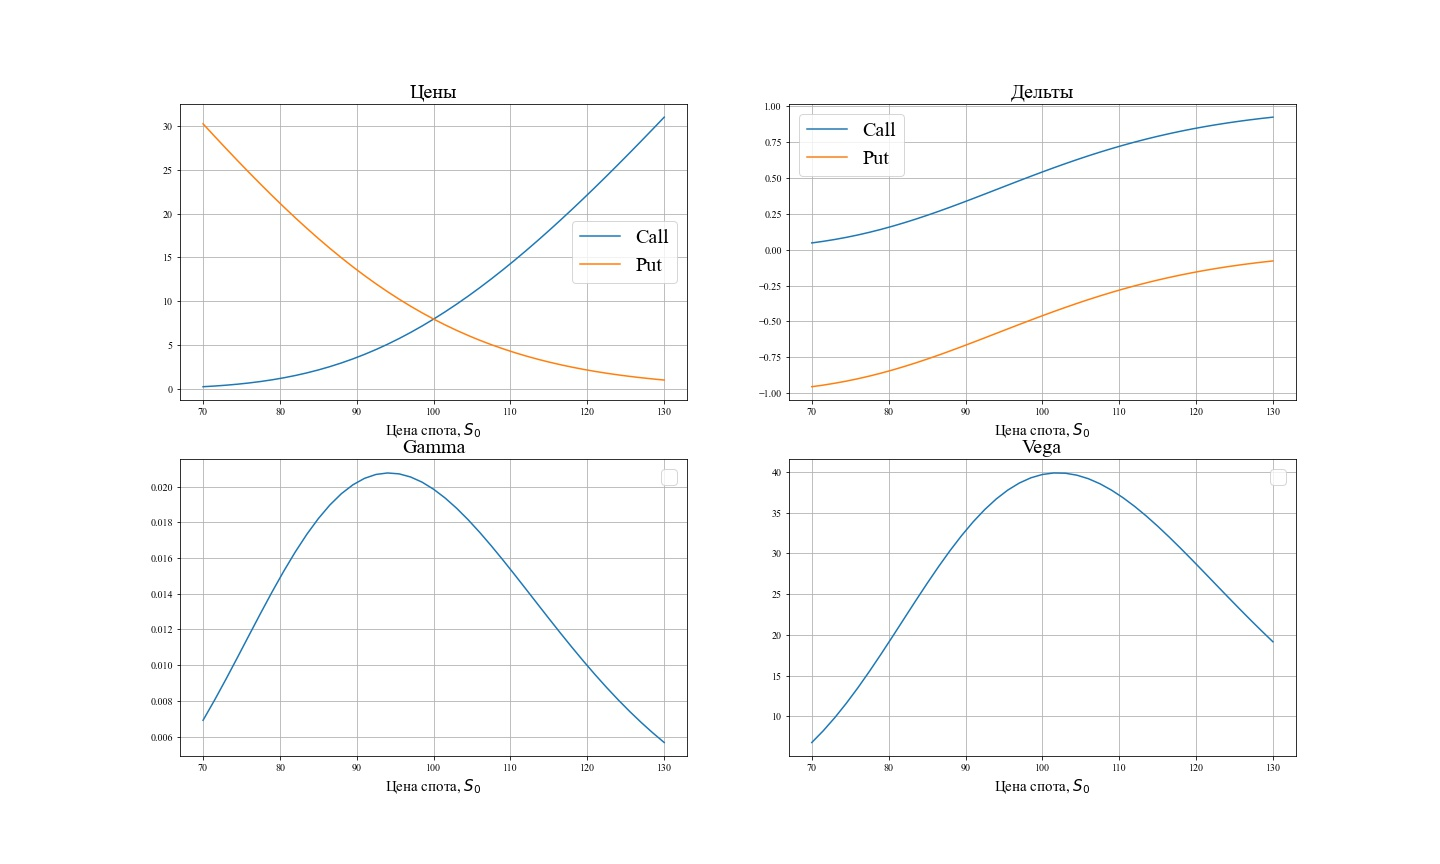
\includegraphics[width=0.9\textwidth]{4_figs/Цены и греки.jpg}}
\end{frame}

\begin{frame}{Свойства}
    \begin{itemize}
        \item<1-> Call-Put parity:
        \begin{align*}
            &S_T - K = (S_T - K)^+ - (K - S_T)^+ \to \\
            &S_t - e^{-r \tau} K = C(t, S_t) - P(t, S_t)
        \end{align*}

        \item<2-> Монотонность по страйку. Если $K_1 < K_2$
        \begin{align*}
               (S_T - K_1) > (S_T - K_2) \to C(t, S_t; K_1) > C(t, S_t; K_2) 
        \end{align*}В частности:
        $$
            C(t, S_t; K) \leq C(t; S_t; 0) = S_t
        $$

        \item<3-> Выпуклость по страйку:
        $$
            \dfrac{\partial^2 C}{\partial K^2} = e^{-r\tau} \mathbb{E}^{\mathbb{Q}} \dfrac{\partial^2}{\partial K^2} (S_T - K)^+ =
            e^{-r\tau} \mathbb{E}^{\mathbb{Q}} \delta(S_T - K) = e^{-r\tau} p(K)
        $$

        \item<4-> Границы:
        $$
            C(t, S_t) = e^{-r\tau}\mathbb{E}^Q (S_T - K)^+ \geq e^{-r\tau} (\mathbb{E}^Q S_T - K)^+ = (S_t - e^{-r\tau} K)^+
        $$
    \end{itemize}    
\end{frame}

\end{document}